\documentclass[11pt]{article}

\usepackage[margin=1in]{geometry}
\usepackage{times}
\usepackage[T1]{fontenc}
\usepackage[utf8]{inputenc}
\usepackage{amsmath,amssymb}
\usepackage{graphicx}
\usepackage{booktabs}
\usepackage{array}
\usepackage{multirow}
\usepackage{hyperref}
\usepackage{cite}
\usepackage{enumitem}
\usepackage{caption}
\usepackage{titlesec}
\usepackage{authblk}

\hypersetup{
    colorlinks=true,
    linkcolor=black,
    citecolor=black,
    urlcolor=blue,
    pdftitle={MoodSync: A Two-Stage Generative Pipeline for Mapping Conversational Affect to Text-Conditioned Music},
    pdfauthor={Dirshak Deepak Patro, Disha Kataria}
}

\titlespacing*{\section}{0pt}{1.4ex plus 1ex minus .2ex}{0.9ex plus .2ex}
\titlespacing*{\subsection}{0pt}{1.2ex plus 1ex minus .2ex}{0.7ex plus .2ex}

\newcommand{\musicgen}{\textsc{MusicGen}}

\title{\textbf{MoodSync: A Two-Stage Generative Pipeline for Mapping Conversational\\ Affect to Text-Conditioned Music, and a Closed-Loop\\ Evaluation of Its Emotional Fidelity}}

\author[1]{Dirshak Deepak Patro}
\author[1]{Disha Kataria}
\affil[1]{Independent Research}

\date{}

\begin{document}

\maketitle

\begin{abstract}
We present MoodSync, a locally-run conversational system that converts free-text descriptions of a user's emotional state into a short, original piece of instrumental music. MoodSync chains two frozen, pretrained foundation models through a small, hand-authored, fully interpretable intermediate layer: a general-purpose large language model (LLM) first reads a user's message and extracts a two-dimensional valence/arousal (V/A) reading grounded in Russell's Circumplex Model of Affect~\cite{russell1980circumplex}, after which a deterministic nearest-neighbor interpolation step maps that coordinate onto a curated bank of ten named emotion regions, each carrying a hand-authored musical descriptor (tempo, instrumentation, dynamics, and mood vocabulary). A templated natural-language generator turns the resulting descriptor into a text prompt, which conditions \musicgen{}~\cite{copet2023musicgen}, a single-stage autoregressive transformer built on the EnCodec neural audio codec~\cite{defossez2022encodec}, to synthesize a 30-second clip. We describe the system's architecture, failure-handling design, and the rationale for keeping the emotion-to-descriptor mapping outside of any learned model. We then report what is, to our knowledge, the first \emph{closed-loop} emotion-consistency evaluation of a V/A-conditioned \musicgen{} pipeline: rather than measuring prompt-text adherence, we render clips for all ten regions and pass them to an independent audio-text model (CLAP~\cite{wu2023clap}) whose probe wording shares no vocabulary with the generation prompts, asking which mood each clip \emph{actually sounds like}. Over 30 clips, the frozen pipeline recovers the intended region 30.0\% of the time against a 10\% chance baseline ($p = 2.0\times10^{-3}$), with 66.7\% valence-sign and 70.0\% arousal-sign agreement and a mean CLAP-to-target similarity of 0.275. The aggregate result conceals a sharp asymmetry: acoustically distinctive high-arousal negative regions are recovered reliably (\emph{angry}, 3/3), while low-arousal and mid-valence regions are recovered not at all (\emph{relaxed}, \emph{hopeful}, \emph{bored}, \emph{anxious}, \emph{exhausted}, all 0/3), and the judge's predictions collapse onto a few labels --- \emph{angry} is chosen for 10 of 30 clips while \emph{relaxed} and \emph{hopeful} are never chosen. We argue this partial-fidelity result, not a headline accuracy figure, is the actionable finding for emotion-conditioned music generation, and we set out a LoRA fine-tuning methodology targeting precisely the regions the measurement identifies as weak.
\end{abstract}

\vspace{0.5em}
\noindent\textbf{Keywords:} text-to-music generation, affective computing, valence-arousal, MusicGen, low-rank adaptation, generative audio evaluation, human-computer interaction

\section{Introduction}

Text-to-music generation has, in the space of roughly two years, moved from a research curiosity into a family of usable, publicly released systems. Autoregressive token-based models such as \musicgen{}~\cite{copet2023musicgen} and MusicLM~\cite{agostinelli2023musiclm}, and diffusion-based systems such as AudioLDM~\cite{liu2023audioldm} and AudioLDM~2~\cite{liu2024audioldm2}, can now synthesize plausible, stylistically coherent instrumental audio from a short natural-language description. This capability opens an interesting application space at the intersection of affective computing and generative audio: systems that do not ask a user to describe music directly, but instead infer an emotional state from something the user says, and let that inferred state --- rather than an explicit musical vocabulary --- drive generation.

MoodSync is our exploration of that space. It is a single-user, locally-run chat application in which a user's free-text message about how they feel is first read by a large language model and converted into a psychologically grounded, continuous two-dimensional coordinate (valence and arousal, following the Circumplex Model of Affect~\cite{russell1980circumplex}), and only then translated --- through a small, fully interpretable, hand-authored intermediate layer --- into a text prompt for \musicgen{}. The system deliberately avoids training or fine-tuning any model for its baseline configuration; all "learning" in the shipped system lives in a ten-region, hand-curated lookup table rather than in model weights, which keeps the mapping auditable and tunable by a human designer without touching model internals.

This choice is a considered trade-off, not an oversight. A zero-shot, prompt-only pipeline is trivial to deploy, requires no GPU, and has no training data to curate --- but it also means the underlying \musicgen{} checkpoint has no specific notion of what \emph{this application's} vocabulary for "relaxed" or "anxious" ought to sound like; it only has the generic associations it acquired from its own pretraining captions. Before assuming that gap matters, however, it should be measured: the second contribution of this paper is a closed-loop evaluation asking how much of the intended emotion actually reaches the audio in the zero-shot configuration (Section~\ref{sec:eval}). Only then do we set out, without running it, what closing the remaining gap through fine-tuning would look like in practice (Section~\ref{sec:finetune}).

\subsection{Contributions}

This paper makes the following contributions:
\begin{enumerate}[leftmargin=*]
    \item We describe the end-to-end architecture of MoodSync, a two-stage generative pipeline that separates emotion \emph{understanding} (an LLM call) from emotion \emph{sonification} (a deterministic, geometrically motivated mapping over a small hand-authored knowledge base), and we argue for the specific benefits of keeping that second stage non-learned.
    \item We detail the system's concurrency, resilience, and failure-handling design, including a three-tier LLM provider cascade and a background-thread-plus-polling architecture for long-running \musicgen{} inference, which we present as a template for other locally-run, single-user generative-audio applications.
    \item We present a closed-loop emotion-consistency evaluation protocol for emotion-conditioned music generation, in which generated audio is judged by an independent audio-text model using probe wording that shares no vocabulary with the generation prompts. This measures whether the intended affect reaches the audio, rather than whether the model rendered the prompt it was given --- a distinction the field's reliance on prompt-adherence CLAP scores obscures, and one that no published \musicgen{} adaptation, including the closest methodological precedent~\cite{lee2026loramusicgen}, has yet reported for its target conditioning variable.
    \item We apply that protocol to the frozen pipeline and report a partial-fidelity result: 30.0\% top-1 region recovery against a 10\% chance baseline ($p = 2.0\times10^{-3}$), with 66.7\% valence-sign and 70.0\% arousal-sign agreement. We show the aggregate conceals a systematic asymmetry --- acoustically extreme regions are recovered perfectly while five of ten regions are never recovered, the judge's predictions collapse onto a few labels, and low-arousal content is misheard as high-arousal --- and we argue this asymmetry, not the headline figure, is what should drive subsequent engineering.
    \item We set out a LoRA fine-tuning methodology~\cite{hu2022lora} for \texttt{facebook/musicgen-small} on the MTG-Jamendo mood/theme subset~\cite{bogdanov2019jamendo}, targeting the text-conditioning pathway and aimed specifically at the regions the evaluation identifies as weak. We deliberately report no results for it: the checkpoint has not been trained, and the measured baseline above is what such a fine-tune would have to beat.
\end{enumerate}

\section{Related Work}

\subsection{Text-to-Music Generation}

Modern text-to-music systems fall broadly into two families. Autoregressive token-based models compress raw audio into discrete tokens with a neural codec and then model those tokens with a transformer language model, conditioned on a text embedding. \musicgen{}~\cite{copet2023musicgen} is the representative system in this family: it operates over four parallel codebooks produced by the EnCodec codec~\cite{defossez2022encodec} at a 50~Hz frame rate, and uses a delay pattern across codebooks so that all four streams can be generated in a single autoregressive pass rather than requiring cascaded upsampling models. MusicLM~\cite{agostinelli2023musiclm} takes a related but distinct approach, using a hierarchical sequence-to-sequence formulation over semantic and acoustic tokens. The second family is diffusion-based: AudioLDM~\cite{liu2023audioldm} and its successor AudioLDM~2~\cite{liu2024audioldm2} operate by denoising a latent representation of audio conditioned on text or other modalities, drawing on the broader success of latent diffusion in image generation. MoodSync's generation stage builds directly on \musicgen{}, using its publicly released, Hugging Face \texttt{transformers}-hosted \texttt{small} checkpoint (approximately 300M parameters) purely at inference time in its baseline configuration.

\subsection{Affective Computing and the Circumplex Model}

Representing emotion as a continuous point in a low-dimensional space, rather than as a member of a fixed discrete label set, has a long history in psychology. Russell's Circumplex Model of Affect~\cite{russell1980circumplex} proposes that affective states can be organized along two largely independent axes --- valence (how negative or positive an experience is) and arousal (how calm or activated it is) --- such that nearby-but-distinct emotions (for instance, anxiety and anger, both negative-valence and high-arousal) occupy nearby but separable regions of the plane rather than disjoint categories. This model has been widely adopted in music-emotion research specifically, since musical affect is itself frequently described along comparable continuous axes rather than through a small closed vocabulary, and it underlies several of the annotated datasets discussed in Section~\ref{sec:datasets}, as well as MoodSync's own ten-region emotion map.

\subsection{Music-Emotion Datasets}
\label{sec:datasets}

Several datasets pair music audio with valence/arousal or mood/theme annotations and are directly relevant to any project that fine-tunes a generative model toward emotion-conditioned output. DEAM~\cite{aljanaki2017deam} provides continuous, time-varying valence/arousal annotations collected via crowdsourcing for a corpus of licensed and Creative-Commons music. PMEmo~\cite{zhang2018pmemo} similarly pairs music with both self-reported and physiologically measured emotional responses. EMOPIA~\cite{hung2021emopia} focuses specifically on solo piano performance, with clip-level annotations across the four quadrants of the valence/arousal plane, and is additionally paired with symbolic (MIDI) representations, making it useful for emotion-conditioned symbolic generation as well as audio-based work. The MTG-Jamendo dataset~\cite{bogdanov2019jamendo}, which the fine-tuning methodology proposed in Section~\ref{sec:finetune} would use, differs from the above in scale and annotation style: it is a large (over 55,000 track), Creative-Commons-licensed collection drawn from the Jamendo platform, annotated across 195 tags spanning genre, instrumentation, and mood/theme categories contributed by content uploaders rather than dedicated annotators. Its mood/theme-tagged subset, introduced for the MediaEval 2019 Emotion and Theme Recognition in Music task, has since become a common substrate for both automatic mood-tagging research and, as in the present work, generative fine-tuning toward emotion-aware music synthesis.

\subsection{Parameter-Efficient Fine-Tuning of Generative Audio Models}

Fully fine-tuning a pretrained generative audio model of even moderate scale is expensive in both compute and data: \musicgen{}-small was pretrained by Meta AI on roughly 20{,}000 hours of licensed music, several orders of magnitude larger than any mood-annotated dataset available for a downstream fine-tune, which makes full fine-tuning on a small dataset prone to catastrophic forgetting and overfitting. Low-Rank Adaptation (LoRA)~\cite{hu2022lora} addresses this by freezing the base model's pretrained weights entirely and injecting small, trainable low-rank update matrices into selected linear layers (most commonly the attention projections), which drastically reduces the number of trainable parameters and the associated memory footprint while retaining most of the base model's general capability. LoRA has already been applied to \musicgen{}-family fine-tuning specifically, including directly to its text-conditioning pathway: the closest published methodological precedent to the present work, Few-shot LoRA tuning for genre-specific music generation with semantic prompt matching~\cite{lee2026loramusicgen}, applies LoRA specifically to \texttt{musicgen-small}'s text encoder --- the same conditioning pathway targeted in this paper --- to build genre-specific adapters (trained and evaluated on jazz and hip-hop subsets of the FMA dataset), together with an automatic adapter-selection mechanism based on cosine similarity between a user's prompt and predefined genre labels in the text-embedding space; that work reports consistent CLAP-based prompt-audio alignment gains over the un-adapted \musicgen{}-small baseline (e.g.\ CLAP rising from 0.3524 to 0.3813 for jazz prompts), but --- like the present evaluation --- relies on CLAP-based prompt adherence rather than a closed-loop, independently-verified check against its actual target conditioning variable (genre, in that case; mood, in ours). A separate study applying LoRA to a diffusion-based music generator reports that a rank-8, alpha-16 configuration improved CLAP score by 7.7\% relative to the un-adapted baseline~\cite{kim2025loradiffusion}, corroborating that modest LoRA ranks are sufficient to produce a measurable prompt-adherence gain in this domain. MoodSync's own fine-tuning methodology (Section~\ref{sec:finetune}) follows the same LoRA-over-frozen-\musicgen{} pattern, applied specifically to the text-conditioning pathway rather than to a new conditioning modality --- the same architectural choice made in~\cite{lee2026loramusicgen}, here targeting mood/theme conditioning rather than genre.

\subsection{Evaluation Metrics for Generative Audio}

Because generative audio produces continuous signals rather than discrete labels, evaluation departs from the accuracy/precision/recall framing standard in classification. Fr\'echet Audio Distance (FAD)~\cite{kilgour2019fad,gui2024fad} measures the distributional distance, in an embedding space, between generated audio and a reference set of real audio, and is the closest audio analogue of the Fr\'echet Inception Distance used for image generation; because it is a set-level distributional statistic computed against a chosen embedding model and reference set, its absolute value is not directly comparable across studies that use different feature extractors or references. CLAP score~\cite{wu2023clap} measures the cosine similarity between a generated clip's audio embedding and its conditioning text's embedding under a Contrastive Language-Audio Pretraining model, on a $[-1,1]$ scale, and is the standard proxy for prompt adherence. Kullback--Leibler divergence between the label-probability distributions an auxiliary audio classifier assigns to generated versus reference audio is used as a proxy for content-level (rather than purely perceptual) similarity. Chroma cosine similarity compares frame-wise 12-dimensional pitch-class profiles between generated audio and a reference, and is used chiefly to assess harmonic and melodic adherence to a target. Mean Opinion Score (MOS), collected from human listeners on a 1--5 scale, remains the field's ground-truth subjective measure, since the field's ultimate goal --- perceived musical and emotional quality --- is not fully captured by any single objective proxy.

For precision, the formal definitions used to compute each metric in Section~5 are given below, with $g$ denoting a generated clip and $r$ a reference (real) clip.

\paragraph{Fr\'echet Audio Distance (FAD).} Given an embedding model $\phi$, let $(\mu_r, \Sigma_r)$ and $(\mu_g, \Sigma_g)$ be the mean and covariance of $\phi$-embeddings computed over a reference set $R$ of real audio and a generated set $G$, respectively. Then
\begin{equation}
\mathrm{FAD}(R, G) = \lVert \mu_r - \mu_g \rVert_2^2 + \mathrm{Tr}\!\left(\Sigma_r + \Sigma_g - 2\left(\Sigma_r \Sigma_g\right)^{1/2}\right),
\label{eq:fad}
\end{equation}
i.e.\ the squared Fr\'echet (2-Wasserstein) distance between the two embedding distributions, treated as multivariate Gaussians; lower values indicate the generated set is distributionally closer to the reference set~\cite{gui2024fad}.

\paragraph{CLAP score.} Given a CLAP audio encoder $E_a$ and text encoder $E_t$,
\begin{equation}
\mathrm{CLAP}(g, t) = \frac{E_a(g) \cdot E_t(t)}{\lVert E_a(g) \rVert \, \lVert E_t(t) \rVert} \in [-1, 1],
\label{eq:clap}
\end{equation}
the cosine similarity between a generated clip's audio embedding and its conditioning text prompt $t$'s embedding under a jointly trained contrastive language-audio model~\cite{wu2023clap}; higher values indicate stronger prompt adherence. The value reported in Table~\ref{tab:results} is the mean of Eq.~\ref{eq:clap} over the evaluation set.

\paragraph{KL divergence.} Given an auxiliary audio classifier that outputs a label-probability distribution $P$ over a fixed label set for a reference clip and $Q$ for the corresponding generated clip,
\begin{equation}
D_{\mathrm{KL}}(P \,\|\, Q) = \sum_{i} P(i) \log \frac{P(i)}{Q(i)},
\label{eq:kl}
\end{equation}
averaged over the evaluation set; lower values indicate the generated audio induces a label distribution closer to that of the reference audio.

\paragraph{Chroma cosine similarity.} Given per-frame 12-dimensional chroma (pitch-class) vectors $c_g[n]$ and $c_r[n]$ for a generated/reference pair aligned over $N$ frames,
\begin{equation}
\mathrm{Chroma}(g, r) = \frac{1}{N} \sum_{n=1}^{N} \frac{c_g[n] \cdot c_r[n]}{\lVert c_g[n] \rVert \, \lVert c_r[n] \rVert} \in [0, 1],
\label{eq:chroma}
\end{equation}
the frame-wise mean cosine similarity between pitch-class profiles; higher values indicate closer harmonic/melodic agreement.

\paragraph{Mean Opinion Score (MOS).} Given ratings $\{ s_{i,j} \in \{1,\dots,5\} \}$ from $N$ listeners each rating $M$ clips,
\begin{equation}
\mathrm{MOS} = \frac{1}{NM} \sum_{i=1}^{N} \sum_{j=1}^{M} s_{i,j},
\label{eq:mos}
\end{equation}
the mean listener-assigned rating across all clips and raters, on a 1 (bad) to 5 (excellent) scale.

None of these five metrics measures whether generated audio conveys an intended emotion. FAD scores distributional realism, chroma similarity scores harmonic agreement with a reference, KL divergence scores agreement between auxiliary-classifier label distributions, and MOS scores perceived quality; CLAP, the only one that considers the conditioning text at all, scores similarity between a clip and \emph{the prompt that generated it}, and so rewards a model for rendering whatever wording it was handed. For an application whose entire claim is that a user's affective state reaches the audio intact, that is a proxy for a proxy. Section~\ref{sec:eval} therefore adapts CLAP into a closed-loop test --- judging each clip against affect probes that share no vocabulary with its generation prompt --- which measures the property directly rather than by proxy.

\section{System Architecture}

\subsection{Overview}

MoodSync is implemented as a single-process Flask web application with no user-account system and no cloud storage beyond an optional hosted LLM call; persistence is local, via SQLite for structured data and the filesystem for generated audio. A user interaction proceeds through five stages, described below:

\begin{enumerate}[leftmargin=*]
    \item \textbf{Emotion extraction.} The user's free-text message is sent to an LLM, which returns a structured JSON object containing a valence score, an arousal score (both clamped to $[-1,1]$), and a short, warm, one-line reply.
    \item \textbf{Region interpolation.} The $(valence, arousal)$ point is mapped onto the two nearest of ten hand-authored named emotion regions via inverse-distance weighting, producing a music descriptor: a tempo range, an instrument list, a dynamics vocabulary, and a mood-word list.
    \item \textbf{Prompt construction.} A templated natural-language generator randomly samples from the descriptor's vocabulary and assembles a free-text prompt suitable for \musicgen{}'s text encoder.
    \item \textbf{Music generation.} The prompt conditions a frozen \texttt{facebook/musicgen-small} checkpoint, which autoregressively generates a 30-second audio clip.
    \item \textbf{Persistence and playback.} The resulting waveform is peak-normalized, quantized to 16-bit PCM, written to disk as a WAV file, and streamed to the browser as an embedded audio player once generation completes.
\end{enumerate}

\subsection{Stage 1: LLM-Based Emotion Extraction}

The emotion-extraction stage uses a general-purpose, instruction-tuned autoregressive transformer decoder rather than a purpose-built sentiment classifier; extraction is achieved entirely through prompt engineering and in-context learning, with no gradient updates and no training data owned by the project for this stage. A single system prompt establishes the model's persona as the emotional-analysis component of a music-therapy chat application and demands strict JSON output matching an exact schema of \texttt{valence}, \texttt{arousal}, and \texttt{reply} fields. Four worked few-shot examples, spanning a deliberate spread of valence/arousal combinations, anchor the model's numeric calibration before it processes the real input, and a low sampling temperature (0.4) favors consistent structured output over creative variation.

Robustness is handled at two levels. First, because language models do not reliably emit bare, well-formed JSON, an extraction routine strips markdown code fences and regex-isolates the first well-formed JSON object in the response before parsing. Second, a validation routine defensively coerces the valence and arousal fields to floating-point numbers, ensures the reply is a non-empty string, and clamps both numeric fields into the required $[-1,1]$ range in case the underlying model overshoots the requested scale.

The stage is implemented as a three-tier provider cascade with graceful degradation: a hosted, low-latency inference API is tried first (an 8-billion-parameter Llama~3.1-Instruct variant; a recent reproducible comparison of this exact model size for structured-extraction tasks reports 73--79\% schema completeness against a proprietary baseline~\cite{nawalny2025llmextraction}), a locally run instance of the same model family is tried on failure or missing configuration, and, if both are unreachable, a hardcoded neutral fallback returns $valence=0$, $arousal=0$, and a generic acknowledgement so that the downstream generation stage is never left without a usable input. Each hosted provider is retried once before the cascade falls through, and the overall extraction function is designed to never raise an exception, catching every failure path internally.

\subsection{Stage 2: Valence/Arousal-to-Descriptor Mapping}

This stage is deliberately rule-based rather than learned: a deterministic geometric algorithm operates over a small, hand-authored knowledge base of ten named emotion regions (relaxed, calm, happy, excited, hopeful, sad, bored, angry, anxious, and exhausted), each defined by a representative $(valence, arousal)$ coordinate and a hand-curated musical descriptor --- a tempo range, a list of characteristic instruments, a list of dynamics adjectives, and a list of mood words --- chosen to match plausible musical conventions for that quadrant of the affective plane (for instance, high-arousal, negative-valence anger is associated with fast, dissonant, percussive descriptors, while low-arousal, positive-valence calm is associated with slow, warm, acoustic ones).

Given a new $(valence, arousal)$ point, the algorithm computes the Euclidean distance to every region's coordinate, retains the two nearest regions $r_1$ (distance $d_1$) and $r_2$ (distance $d_2$), and computes an inverse-distance blend weight
\begin{equation}
w_1 = \frac{1/d_1}{1/d_1 + 1/d_2},
\end{equation}
falling back to $w_1 = 1$ when the input point lands almost exactly on a single region. The descriptor's vocabulary fields (instruments, dynamics, mood words) are taken as the deduplicated union of both regions' lists, while the tempo range is taken specifically from the primary (nearest) region. This is, in effect, a $k=2$ nearest-neighbor lookup with inverse-distance weighting over a small, hand-labeled two-dimensional reference set --- chosen because ten hand-curated regions are sufficient to cover the affective plane smoothly for this application's purposes, and because no labeled training data exists (prior to the fine-tuning work in Section~\ref{sec:finetune}) to justify a learned regression or classification model in its place.

\subsection{Stage 3: Prompt Construction}

The descriptor dictionary produced by Stage~2 is converted into free-text via templated natural-language generation: three mood words, three instruments, and two dynamics adjectives are randomly sampled from the descriptor's deduplicated lists, and four sentence-fragment templates (covering the opener, the instrumentation clause, the dynamics clause, and the tempo clause) are randomly selected and joined into a single prompt string. Randomizing both the sampled vocabulary and the template selection ensures that repeated messages landing in the same emotional region do not always produce an identical prompt, and therefore not an identical-sounding clip. This lightweight, template-based approach is a deliberate substitute for a learned natural-language generator: because the target vocabulary is small, controlled, and domain-specific, hand-written templates are more reliable and more controllable than an additional LLM call in this position, and they avoid introducing a third external API dependency into the generation critical path.

\subsection{Stage 4: Text-to-Music Generation}

The core generative component is \texttt{facebook/musicgen-small}, loaded through Hugging Face \texttt{transformers}' \texttt{MusicgenForConditionalGeneration} class rather than Meta's original \texttt{audiocraft} training codebase, since \texttt{audiocraft} hard-pins an older PyTorch release that has no wheels for the project's Python~3.12 environment; the \texttt{transformers} implementation is a checkpoint-compatible reimplementation of the identical pretrained weights and architecture. Architecturally, \musicgen{} conditions a decoder-only transformer --- built on the self-attention mechanism common to nearly all modern sequence models~\cite{vaswani2017attention} --- on text embeddings from a frozen T5-based encoder~\cite{raffel2020t5}, and autoregressively predicts discrete acoustic tokens produced by the EnCodec neural audio codec~\cite{defossez2022encodec}, which compresses and reconstructs raw waveforms much as a VQ-VAE-style tokenizer~\cite{oord2017vqvae} discretizes continuous signals for language-model-style sequence modeling. A fixed inter-codebook delay pattern lets \musicgen{}'s four parallel codebooks be generated in a single autoregressive pass rather than requiring a cascaded upsampling model~\cite{copet2023musicgen}.

At inference time, the model and processor are lazily loaded exactly once behind a threading lock (a module-level singleton pattern), moved to GPU if available, and set to evaluation mode. Given a text prompt and a target duration, the number of tokens to generate is computed from \musicgen{}'s known $\sim$50~Hz codec frame rate (1{,}500 tokens for the application's fixed 30-second clips), and generation runs inside a no-gradient context for memory efficiency. A separate module-level lock serializes all generation calls system-wide, since the workload is compute-bound and concurrent generation requests would only slow each other down rather than run in parallel usefully. The generated tensor is peak-normalized to 95\% of full scale to avoid clipping while leaving headroom, quantized to 16-bit signed PCM, and written directly to a WAV file with no intermediate codec transcoding step, keeping the dependency footprint minimal and the output universally playable in a browser.

\subsection{Concurrency and Resilience}

Because \musicgen{} inference on CPU can take on the order of minutes for a 30-second clip, the LLM round trip (Stages~1--3, which complete quickly) is executed synchronously within the HTTP request, while generation (Stage~4) is dispatched to a background daemon thread; the HTTP response returns immediately with the assistant message marked \texttt{generating}, and the frontend polls a status endpoint roughly every 2.5 seconds until the status transitions to \texttt{done} or \texttt{error}. This background-thread-plus-polling design was chosen over synchronous blocking (to avoid multi-minute HTTP timeouts) and over WebSockets (unnecessary complexity for a single-user local application, for which a plain interval poll is sufficient).

Resilience is layered at every external-dependency boundary. The LLM stage's three-tier provider cascade, described above, guarantees the pipeline always receives a usable emotional reading even with zero configured API keys and no network access beyond the initial \musicgen{} weight download. The generation stage wraps all inference in a try/except block inside the background thread, logging a full traceback server-side and reflecting any failure to the user as a clear, non-blocking error state rather than leaving the interface stuck on a generating indicator indefinitely. On every server startup, any message still marked \texttt{generating} --- necessarily orphaned from a previous process that terminated mid-generation --- is proactively swept to an error state, since such a message can never complete on its own. Every database operation opens and closes its own short-lived SQLite connection, which is what makes the persistence layer safe to call concurrently from both request-handling threads and the separate background generation thread without an explicit connection pool.

\subsection{Design Rationale}

The system's central methodological choice is to separate "understand the emotion" (Stage~1, an LLM call) from "decide what that emotion sounds like" (Stage~2, a deterministic lookup) rather than asking a single LLM call to produce a music-description prompt directly. This keeps the emotion-to-music mapping auditable and hand-tunable --- a designer can edit a YAML configuration file to change the musical character associated with a given region without touching any model --- and insulates the mapping from any particular LLM's stylistic quirks or hallucination risk when describing music. Grounding the interpolation in an established psychological model (the Circumplex Model of Affect~\cite{russell1980circumplex}) rather than an ad hoc taxonomy gives the two-dimensional interpolation a theoretical basis rather than an arbitrary one. Finally, because no model in the baseline configuration is trained or fine-tuned, the entire "learning" surface of the shipped system is the human-editable YAML descriptor table, not any set of model weights --- a design that is simple to reason about and cheap to deploy, at the cost of leaving \musicgen{}'s associations between the application's specific vocabulary and its intended emotional targets entirely generic. That cost is the motivation for the fine-tuning work described next.

\section{Closed-Loop Evaluation of the Zero-Shot Pipeline}
\label{sec:eval}

\subsection{Motivation: Prompt Adherence Is Not Emotional Fidelity}

The standard proxy for conditioning quality in text-to-music work is CLAP score~\cite{wu2023clap}: the cosine similarity between a generated clip's audio embedding and its own conditioning prompt's text embedding. This measures whether the model rendered \emph{the prompt it was given}. For MoodSync, that is the wrong question. The system's claim is not that it renders its prompts faithfully but that a user's emotional state survives a four-step journey --- message $\to$ LLM $\to$ V/A coordinate $\to$ descriptor $\to$ prompt $\to$ audio --- and arrives recognizable. A pipeline could achieve a high CLAP score while mapping every emotion onto music that no listener would describe as matching it, simply because the descriptor vocabulary itself is a poor proxy for felt affect.

We therefore evaluate the property the application actually depends on. As noted in Section~2.4, the closest published methodological precedent for text-encoder-targeted LoRA adaptation of \musicgen{}~\cite{lee2026loramusicgen} verifies its own conditioning target (genre) only through CLAP prompt-audio similarity, not through an independent classifier; to our knowledge no published \musicgen{} adaptation has reported a closed-loop check against its target conditioning variable. The evaluation below is, to our knowledge, the first such check for mood.

\subsection{Protocol}

For each of the ten named regions we ran the \emph{deployed} pipeline unchanged --- the same \texttt{map\_va\_to\_descriptor} and \texttt{build\_prompt} functions the running application calls --- to render three 30-second clips from the region's own $(valence, arousal)$ coordinate, giving $n = 30$ clips from the frozen \texttt{facebook/musicgen-small} checkpoint. Prompt randomization (Section~3.3) was left enabled, so the three clips per region differ in sampled vocabulary and sentence template, as they would in production.

Each clip was then embedded with CLAP (\texttt{laion/clap-htsat-unfused}) and compared against ten text probes, one per region, by cosine similarity; the highest-scoring probe is the predicted mood. The critical design choice is that \textbf{the probes share no vocabulary with the generation prompts}. Probes are bare affect terms (\emph{``anxious, uneasy music''}, \emph{``weary, drained music''}) containing no instrument, dynamics, or tempo words, whereas generation prompts are built entirely from instrument, dynamics, tempo, and mood-word lists. A correct match therefore cannot be obtained by echoing prompt surface form; it requires that the audio itself carry the affect. This makes the test strictly harder than a CLAP prompt-adherence score, and it is why the numbers below are not comparable to published CLAP figures for prompt adherence.

Because the judge is independent of the generator, this measures the pipeline end-to-end rather than any single component --- a property we return to in Section~\ref{sec:eval-limits}, since it also means a failure cannot be attributed to the generator alone.

\subsection{Results}

Table~\ref{tab:results} reports the aggregate metrics. The pipeline recovers the intended region in 9 of 30 clips (30.0\%) against a 10\% chance baseline, which a one-sided binomial test rejects at $p = 2.0 \times 10^{-3}$. Valence-sign and arousal-sign agreement --- whether the judged mood falls in the correct half-plane, a weaker but more forgiving criterion that credits confusing \emph{anxious} with \emph{angry} while still penalizing confusing \emph{calm} with \emph{angry} --- reach 66.7\% and 70.0\% against a 50\% baseline. Both signs are simultaneously correct (correct quadrant) for 14 of 30 clips, against a 25\% chance baseline.

\begin{table}[t]
\centering
\caption{Closed-loop emotion-consistency results for the frozen \texttt{musicgen-small} pipeline, $n = 30$ clips. $p$-values are one-sided binomial tests against the stated chance baseline. Mean CLAP-to-target is the similarity to the clip's \emph{own} region probe, not to its generation prompt, and is therefore not comparable to published prompt-adherence CLAP scores.}
\label{tab:results}
\small
\begin{tabular}{@{}p{5.4cm}p{2.0cm}p{2.0cm}p{3.0cm}@{}}
\toprule
Metric & Value & Chance & Significance \\
\midrule
Top-1 region accuracy & 30.0\% (9/30) & 10.0\% & $p = 2.0\times10^{-3}$ \\
Valence sign agreement & 66.7\% (20/30) & 50.0\% & $p = 0.049$ \\
Arousal sign agreement & 70.0\% (21/30) & 50.0\% & $p = 0.021$ \\
Correct quadrant (both signs) & 46.7\% (14/30) & 25.0\% & --- \\
Mean CLAP-to-target similarity & 0.275 & --- & --- \\
Valence MAE & 0.413 & --- & --- \\
Arousal MAE & 0.503 & --- & --- \\
\bottomrule
\end{tabular}
\end{table}

The pipeline thus transmits emotional information at roughly three times chance, but recovers the specific intended region in fewer than one clip in three. Both conclusions matter, and reporting only the first would misrepresent the system.

\subsection{Where the Signal Survives, and Where It Does Not}

The aggregate figure conceals a sharp and systematic asymmetry. Figure~\ref{fig:confusion} gives the full confusion matrix, and Table~\ref{tab:perregion} the per-region breakdown.

\begin{table}[t]
\centering
\caption{Per-region top-1 accuracy (3 clips each), and how often each label was \emph{chosen} by the judge across all 30 clips. A uniform judge would select each label 3 times.}
\label{tab:perregion}
\small
\begin{tabular}{@{}lcc|lcc@{}}
\toprule
Region & Correct & Times chosen & Region & Correct & Times chosen \\
\midrule
angry     & 3/3 & 10 & sad       & 1/3 & 2 \\
calm      & 2/3 & 5  & relaxed   & 0/3 & 0 \\
happy     & 2/3 & 3  & hopeful   & 0/3 & 0 \\
excited   & 1/3 & 1  & bored     & 0/3 & 1 \\
          &     &    & anxious   & 0/3 & 6 \\
          &     &    & exhausted & 0/3 & 2 \\
\bottomrule
\end{tabular}
\end{table}

\begin{figure}[t]
\centering
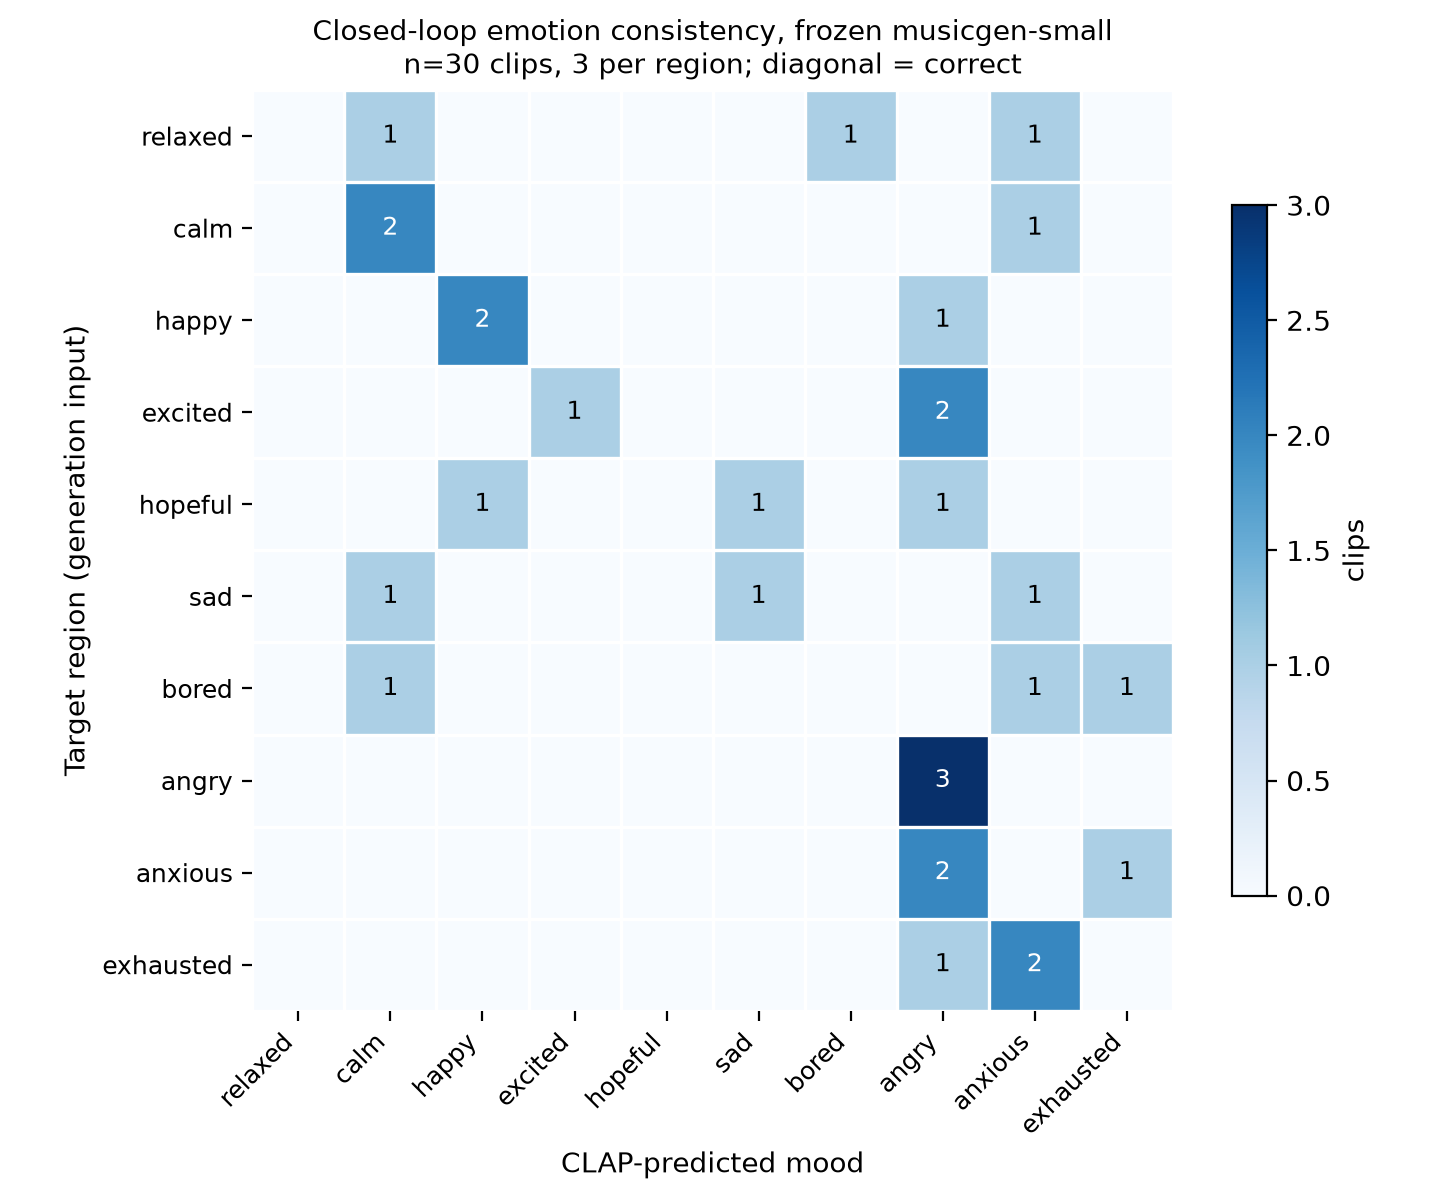
\includegraphics[width=0.86\textwidth]{diagrams/confusion_matrix.png}
\caption{Closed-loop confusion matrix. Rows are the target region used to generate the clip; columns are the mood an independent CLAP judge assigned. The diagonal is correct. Note the density of the \emph{angry} column and the empty \emph{relaxed} and \emph{hopeful} columns.}
\label{fig:confusion}
\end{figure}

Three patterns are visible, and they point in the same direction.

\paragraph{Acoustically distinctive regions survive; subtle ones do not.} \emph{Angry} is recovered perfectly (3/3). Its descriptor is the most acoustically extreme in the bank --- distorted synth bass, heavy drums, 130--150~bpm --- and those properties are exactly what a contrastive audio-text model keys on. \emph{Calm} (2/3) and \emph{happy} (2/3) likewise carry unambiguous signatures. By contrast \emph{relaxed}, \emph{hopeful}, \emph{bored}, \emph{anxious}, and \emph{exhausted} are recovered in 0 of 3 clips each. These are precisely the regions whose descriptors differ from their neighbours in degree rather than kind: \emph{relaxed} and \emph{calm} share warm, slow, acoustic vocabulary, and \emph{bored} and \emph{exhausted} share sparse, low, muted vocabulary. The V/A plane distinguishes them; the rendered audio, as heard by an independent judge, does not.

\paragraph{The judge's predictions collapse onto a few labels.} \emph{Angry} is selected for 10 of 30 clips and \emph{anxious} for 6, while \emph{relaxed} and \emph{hopeful} are never selected at all. The effective label space is therefore closer to eight than ten, and a third of all judgments land on a single label. This inflates \emph{angry}'s apparent success and suppresses everything competing with it, so per-region accuracies should not be read independently of this prior.

\paragraph{Low-arousal negative content is misread as high-arousal tense content.} All three \emph{exhausted} clips (arousal $-0.9$) were judged \emph{anxious} or \emph{angry} (arousal $+0.7$, $+0.8$) --- a complete sign inversion on the axis the descriptor most directly encodes, since \emph{exhausted}'s prompt specifies 45--60~bpm and ``weighted, sparse'' dynamics. The same inversion affects \emph{relaxed} and \emph{bored}. Slow, sparse, low-register audio is being heard as tense rather than depleted, which suggests the failure is concentrated in the arousal axis at its negative extreme rather than distributed evenly.

Taken together, the pipeline reliably conveys \emph{intensity} when intensity is extreme, and conveys little else. This is a far more actionable diagnosis than an aggregate accuracy figure: it identifies which five regions a fine-tune would need to fix, and it predicts that adding training data for \emph{angry} --- the region that already works --- would be wasted effort.

\subsection{Limitations}
\label{sec:eval-limits}

\begin{enumerate}[leftmargin=*]
    \item \textbf{The generator and the judge cannot be separated.} A 0/3 region means the target did not survive the round trip; it does not establish \emph{where} it was lost. \musicgen{} may have failed to render the mood, or CLAP may be unable to hear it. CLAP is trained on general audio captions and is known to be stronger on instrumentation and genre than on fine-grained affect, and the label-collapse above is itself evidence of judge bias. Distinguishing these requires a second, architecturally different judge or a human listening study; we regard this as the single most important gap in the present evaluation.
    \item \textbf{$n = 30$ is small.} The 95\% confidence interval on the headline 30.0\% figure is approximately $[13.6\%, 46.4\%]$. The interval excludes chance, so the above-chance conclusion is safe, but per-region cells rest on 3 clips each and individual rates such as \emph{calm}'s 2/3 should be read as indicative only.
    \item \textbf{Single-checkpoint, single-judge.} All results use \texttt{musicgen-small} and one CLAP checkpoint. Whether the asymmetry is a property of this model size, of this judge, or of the descriptor bank is not established here.
    \item \textbf{Region coordinates are used as inputs, not real user messages.} We drive the pipeline from each region's own $(valence, arousal)$ coordinate, isolating Stages~2--4. This deliberately excludes Stage~1: any error the LLM makes in reading a genuine user message is additional to the loss measured here, so these figures are an upper bound on end-to-end performance from real input.
    \item \textbf{No fine-tuned comparison.} Section~\ref{sec:finetune} sets out a fine-tuning methodology but reports no trained checkpoint; the numbers above characterize the frozen baseline only. They are the baseline against which such a fine-tune would be measured, which is precisely what the evaluation was built to provide.
\end{enumerate}

\section{Proposed Fine-Tuning Methodology}
\label{sec:finetune}

\subsection{Motivation and Conditioning Target}

The zero-shot pipeline described in Section~3 steers \musicgen{} purely through prompt wording; the model has no application-specific notion of what "relaxed" or "anxious" are meant to sound like beyond the generic associations it acquired from its own pretraining captions, so all output-to-intended-emotion fidelity is uncontrolled. Two fine-tuning targets are possible. The lower-effort option is to fine-tune on richer, more consistent text captions drawn from the application's own descriptor vocabulary and prompt phrasing, leaving the existing text-conditioning architecture unchanged. The architecturally deeper option is to add a direct continuous $(valence, arousal)$ conditioning pathway --- for instance a small learned projection into \musicgen{}'s existing cross-attention conditioning space, in the spirit of its optional melody-conditioning mechanism --- which would remove the current pipeline's language bottleneck (numbers~$\to$~words~$\to$~numbers again) but requires modifying the model's conditioning modules rather than only its training data. This paper adopts the text-caption option, applying LoRA to \musicgen{}'s text-conditioning pathway in the same way as the closest published methodological precedent~\cite{lee2026loramusicgen} (which targets genre rather than mood/theme conditioning), and treats direct valence/arousal conditioning as future work.

\subsection{Fine-Tuning Method and Hyperparameters}

In the proposed configuration the base \texttt{facebook/musicgen-small} checkpoint (approximately 300M parameters) would be kept frozen, and Low-Rank Adaptation~\cite{hu2022lora} applied to the attention projection layers of \musicgen{}'s T5-based text encoder~\cite{raffel2020t5} via Hugging Face's \texttt{peft} library~\cite{mangrulkar2022peft}, following the same parameter-efficient, text-encoder-targeted pattern used in the closest published methodological precedent for LoRA-adapted MusicGen fine-tuning~\cite{lee2026loramusicgen}. The decoder transformer and the EnCodec tokenizer would be left entirely frozen. Table~\ref{tab:hyperparams} summarizes the proposed configuration.

\begin{table}[t]
\centering
\caption{LoRA fine-tuning hyperparameters.}
\label{tab:hyperparams}
\begin{tabular}{@{}ll@{}}
\toprule
Parameter & Value \\
\midrule
Base model & \texttt{facebook/musicgen-small} (frozen) \\
LoRA rank ($r$) & 16 \\
LoRA alpha & 32 \\
Batch size & 4 \\
Learning rate & $1 \times 10^{-4}$ \\
Epochs & 10 \\
\bottomrule
\end{tabular}
\end{table}

\subsection{Frozen vs.\ Trainable Components}
\label{sec:frozen}

Because the fine-tuning stage touches only part of the overall MoodSync pipeline, Table~\ref{tab:frozen} makes explicit, component by component, what the proposed fine-tune would update and what would remain frozen throughout --- both in the baseline zero-shot system (Section~3, which is what the evaluation in Section~\ref{sec:eval} actually measures) and in the LoRA configuration described above.

\begin{table}[t]
\centering
\caption{Frozen vs.\ trainable status of every component in the pipeline. Only the LoRA adapter matrices would be updated by gradient descent; every other component is either a frozen pretrained network or a non-learned, hand-authored rule. No checkpoint was trained for this paper.}
\label{tab:frozen}
\small
\begin{tabular}{@{}p{4.6cm}p{2.1cm}p{6.3cm}@{}}
\toprule
Component & Status & Notes \\
\midrule
LLM emotion extraction (Stage~1) & Frozen & Pretrained LLM used purely via prompting; zero gradient updates at any point. \\
Valence/arousal $\to$ descriptor mapping (Stage~2) & Frozen / non-learned & Deterministic $k{=}2$ nearest-neighbor lookup over a hand-authored table; never trained. \\
Prompt construction (Stage~3) & Frozen / non-learned & Templated natural-language generation; never trained. \\
\musicgen{} text encoder (T5-based), non-attention sublayers & Frozen & Base pretrained weights unchanged; LoRA does not wrap these sublayers. \\
\musicgen{} decoder transformer (all sublayers) & Frozen & Would receive no gradient at any point. \\
\musicgen{} text-encoder attention projection layers (query/value projections) & Frozen base weights, \textbf{augmented} & Base weights frozen; each targeted projection $W$ is augmented with a parallel low-rank update (Eq.~\ref{eq:lora}). \\
LoRA adapter matrices $A, B$ ($r=16$, $\alpha=32$) & \textbf{Trainable} & The \emph{only} parameters that would be updated by gradient descent. \\
EnCodec audio tokenizer & Frozen & Used only to produce target discrete tokens from training audio; not fine-tuned. \\
\bottomrule
\end{tabular}
\end{table}

For a targeted attention-projection weight matrix $W \in \mathbb{R}^{d \times k}$, LoRA freezes $W$ and adds a low-rank update:
\begin{equation}
W' = W + \frac{\alpha}{r} B A, \qquad B \in \mathbb{R}^{d \times r},\; A \in \mathbb{R}^{r \times k},
\label{eq:lora}
\end{equation}
where only $A$ and $B$ receive gradients; $W$ itself is never modified in place, so the original pretrained checkpoint remains recoverable simply by discarding the adapter. With $r=16$ against \texttt{musicgen-small}'s $d=1024$ attention projections, each targeted $1024 \times 1024$ matrix (1{,}048{,}576 parameters) is replaced by $2 \times 1024 \times 16 = 32{,}768$ trainable parameters --- a $32\times$ reduction relative to full fine-tuning of that projection --- which is what keeps the method tractable on the same modest hardware budget that motivated using \texttt{musicgen-small} over its Medium/Large siblings in the first place.

A rank-to-alpha ratio of 1:2 (rank 16, alpha 32) is a common configuration for music/audio LoRA fine-tunes, and comparable settings have been reported elsewhere in this domain, including a rank-8, alpha-16 configuration for a diffusion-based music LoRA study that achieved a 7.7\% CLAP-score improvement over its un-adapted baseline~\cite{kim2025loradiffusion}. A batch size of 4 is modest but expected given that a 30-second clip, once tokenized at \musicgen{}'s $\sim$50~Hz codec frame rate, occupies 1{,}500 tokens per codebook, making VRAM rather than hyperparameter philosophy the binding constraint. Ten epochs on a LoRA adapter (as opposed to a full fine-tune) is on the higher side but not unusual for a single-domain dataset; the principal risk at this epoch count is the adapter overfitting to a narrow slice of the MTG-Jamendo tag vocabulary, which is why validation-loss tracking through the final epoch --- rather than training loss alone --- is the appropriate diagnostic.

\subsection{Dataset}

Training data is drawn from the mood/theme-tagged subset of MTG-Jamendo~\cite{bogdanov2019jamendo}, a Creative-Commons-licensed corpus whose tags were contributed by content uploaders rather than dedicated annotators. To align training captions with the exact phrasing the model will see at inference time, each clip's mood/theme tags should be passed through the same descriptor-mapping and prompt-construction functions used by the deployed pipeline (Stages~2--3 of Section~3), so that every training caption is drawn from the same template and vocabulary distribution the fine-tuned model will subsequently be prompted with in production; this alignment between training-caption style and inference-prompt style is the single largest lever for making the fine-tune pay off.

\section{Discussion}

The evaluation in Section~\ref{sec:eval} changes what can honestly be claimed for a system like MoodSync, and we think the change is instructive beyond this particular application.

The pipeline works, in the narrow and specific sense that emotional information demonstrably survives the round trip from a valence/arousal coordinate to audio and back out through an independent judge, at roughly three times chance. It does not work in the sense a user would care about: presented with a clip generated for \emph{hopeful}, an independent listener model is more likely to call it something else than to call it hopeful. Both of these are true simultaneously, and a paper reporting only the first would be misleading in exactly the way the generative-audio literature's reliance on prompt-adherence metrics invites. A high CLAP score against one's own prompt is compatible with near-total failure at the task the prompt was a proxy for.

The asymmetry is the more useful result. The regions that survive --- \emph{angry} above all --- are those whose musical descriptors differ from their neighbours categorically: distorted bass and 140~bpm drums are not a more intense version of felt piano, they are a different kind of sound. The regions that fail are those separated from their neighbours by degree: \emph{relaxed} versus \emph{calm}, \emph{bored} versus \emph{exhausted}. This suggests the ten-region bank is over-specified relative to what \musicgen{} can actually distinguish. A designer reading Table~\ref{tab:perregion} would be justified in merging the regions that never separate, and would gain more from that one-line configuration change than from any amount of prompt-wording refinement. That is precisely the kind of actionable conclusion the non-learned, hand-editable mapping layer of Section~3.7 was designed to make possible: the fix is a YAML edit, not a retraining run.

The arousal inversion deserves particular attention. Every \emph{exhausted} clip was judged high-arousal despite a descriptor explicitly specifying 45--60~bpm and sparse, weighted dynamics. If \musicgen{} is faithfully rendering slow, sparse, low-register audio and the judge is hearing tension in it, then the language bottleneck discussed in Section~\ref{sec:finetune} is not the binding constraint --- the descriptor vocabulary is reaching the audio, and the failure is one of interpretation. If instead \musicgen{} is not rendering the specified tempo and dynamics, the bottleneck is real and a text-conditioning fine-tune is well targeted. The present evaluation cannot distinguish these, which is why Section~\ref{sec:eval-limits} names a second, architecturally distinct judge as the highest-value next measurement rather than the fine-tune itself. Running the fine-tune first would risk optimizing against a judge's blind spot.

This also reframes the choice between the two fine-tuning targets of Section~\ref{sec:finetune}. The text-caption route leaves the language bottleneck intact; the direct continuous $(valence, arousal)$ conditioning route removes it. The measured failure concentrated at the negative extreme of the arousal axis is at least suggestive that the numbers-to-words-to-numbers round trip is losing information where the axis is most compressed --- \emph{bored}, \emph{exhausted}, and \emph{relaxed} all occupy a narrow band of low-arousal vocabulary. If a follow-up measurement confirms that \musicgen{} is rendering the descriptors faithfully, the language bottleneck is exonerated and effort should go to the descriptor bank instead; if it confirms the descriptors are not surviving into audio, direct conditioning becomes the better investment. Either way the measurement should precede the engineering, which is the opposite of the order this project originally took.

\section{Conclusion}

We have described MoodSync, a locally-run system that converts free-text emotional expression into original instrumental music through a two-stage generative pipeline: a large language model performs psychologically grounded emotion extraction, and a small, deterministic, hand-authored mapping --- rather than any learned model --- translates the resulting valence/arousal coordinate into a text prompt for \musicgen{}. We argued that keeping this intermediate layer non-learned is a deliberate and defensible design choice for a system of this scope, trading model-level customization for auditability and zero-training-infrastructure deployment.

We then reported what is, to our knowledge, the first closed-loop emotion-consistency evaluation of a V/A-conditioned \musicgen{} pipeline: rather than measuring adherence to the prompt the model was given, we asked an independent audio-text model, using probe wording disjoint from the generation prompts, which mood each generated clip actually sounds like. The frozen pipeline recovers the intended region 30.0\% of the time against a 10\% baseline ($p = 2.0\times10^{-3}$), with 66.7\% valence-sign and 70.0\% arousal-sign agreement --- above chance, and well short of reliable. The aggregate conceals a sharp asymmetry that is the paper's most useful finding: acoustically extreme regions are recovered perfectly while five of ten regions are never recovered at all, the judge's predictions collapse onto a handful of labels, and low-arousal content is systematically misheard as high-arousal. We have set out a LoRA fine-tuning methodology aimed at the regions this measurement identifies as weak, and deliberately report no results for it, since the checkpoint has not been trained.

The clearest next steps follow directly from the limitations in Section~\ref{sec:eval-limits}: a second, architecturally distinct judge or a human listening study to separate generator failure from judge blindness; a larger evaluation set to tighten per-region estimates beyond three clips; and an end-to-end variant driven by real user messages rather than region coordinates, which would fold in the Stage~1 extraction error the present protocol excludes by construction. Only once those are in place does training the proposed adapter become a measurement rather than a hope. We would emphasize, as the general lesson, that this ordering --- measure the frozen baseline against the property the application actually depends on, then fine-tune --- is cheap, and that adopting prompt-adherence metrics as a stand-in for conditioning fidelity can conceal exactly the failures that matter most.

\section*{Acknowledgments}

The authors thank Meta AI for publicly releasing the \musicgen{} weights, and the maintainers of the Hugging Face \texttt{transformers} and \texttt{peft} projects, whose inference and parameter-efficient fine-tuning tooling this work builds on. Note that the original \texttt{audiocraft} training codebase was not used; see Section~3.4. Evaluation used the LAION CLAP checkpoint~\cite{wu2023clap} as an independent judge.

\section*{Reproducibility}

The system, the evaluation harness, and the raw results underlying every number in Table~\ref{tab:results} and Table~\ref{tab:perregion} are available at \url{https://github.com/dirshak/MoodSync}. The evaluation is a single command (\texttt{python eval/closed\_loop\_eval.py}) and completes in approximately fifteen minutes on one T4 GPU; \texttt{eval/results.json} contains the per-clip prompts, predictions, and full ten-way similarity vectors, so the confusion matrix and every reported statistic can be recomputed without re-running generation. A hosted demonstration of the system runs at \url{https://huggingface.co/spaces/Stella802/MoodSync}.


\begin{thebibliography}{99}

\bibitem{russell1980circumplex}
J.~A. Russell, ``A circumplex model of affect,'' \emph{Journal of Personality and Social Psychology}, vol.~39, no.~6, pp.~1161--1178, 1980.

\bibitem{copet2023musicgen}
J.~Copet, F.~Kreuk, I.~Gat, T.~Remez, D.~Kant, G.~Synnaeve, Y.~Adi, and A.~D\'efossez, ``Simple and controllable music generation,'' in \emph{Advances in Neural Information Processing Systems (NeurIPS)}, 2023.

\bibitem{agostinelli2023musiclm}
A.~Agostinelli, T.~I. Denk, Z.~Borsos, J.~Engel, M.~Verzetti, A.~Caillon, Q.~Huang, A.~Jansen, A.~Roberts, M.~Tagliasacchi, M.~Sharifi, N.~Zeghidour, and C.~Frank, ``MusicLM: Generating music from text,'' \emph{arXiv preprint arXiv:2301.11325}, 2023.

\bibitem{defossez2022encodec}
A.~D\'efossez, J.~Copet, G.~Synnaeve, and Y.~Adi, ``High fidelity neural audio compression,'' \emph{Transactions on Machine Learning Research (TMLR)}, 2023.

\bibitem{vaswani2017attention}
A.~Vaswani, N.~Shazeer, N.~Parmar, J.~Uszkoreit, L.~Jones, A.~N. Gomez, {\L}.~Kaiser, and I.~Polosukhin, ``Attention is all you need,'' in \emph{Advances in Neural Information Processing Systems (NeurIPS)}, 2017.

\bibitem{raffel2020t5}
C.~Raffel, N.~Shazeer, A.~Roberts, K.~Lee, S.~Narang, M.~Matena, Y.~Zhou, W.~Li, and P.~J. Liu, ``Exploring the limits of transfer learning with a unified text-to-text transformer,'' \emph{Journal of Machine Learning Research}, vol.~21, no.~140, pp.~1--67, 2020.

\bibitem{oord2017vqvae}
A.~van~den Oord, O.~Vinyals, and K.~Kavukcuoglu, ``Neural discrete representation learning,'' in \emph{Advances in Neural Information Processing Systems (NeurIPS)}, 2017.

\bibitem{liu2023audioldm}
H.~Liu, Z.~Chen, Y.~Yuan, X.~Mei, X.~Liu, D.~Mandic, W.~Wang, and M.~D. Plumbley, ``AudioLDM: Text-to-audio generation with latent diffusion models,'' in \emph{Proceedings of the 40th International Conference on Machine Learning (ICML)}, 2023.

\bibitem{liu2024audioldm2}
H.~Liu, Y.~Yuan, X.~Liu, X.~Mei, Q.~Kong, Q.~Tian, Y.~Wang, W.~Wang, Y.~Wang, and M.~D. Plumbley, ``AudioLDM 2: Learning holistic audio generation with self-supervised pretraining,'' \emph{IEEE/ACM Transactions on Audio, Speech, and Language Processing}, vol.~32, pp.~2871--2883, 2024.

\bibitem{hu2022lora}
E.~J. Hu, Y.~Shen, P.~Wallis, Z.~Allen-Zhu, Y.~Li, S.~Wang, L.~Wang, and W.~Chen, ``LoRA: Low-rank adaptation of large language models,'' in \emph{International Conference on Learning Representations (ICLR)}, 2022.

\bibitem{mangrulkar2022peft}
S.~Mangrulkar, S.~Gugger, L.~Debut, Y.~Belkada, S.~Paul, and B.~Bossan, ``PEFT: State-of-the-art parameter-efficient fine-tuning methods,'' \url{https://github.com/huggingface/peft}, 2022.

\bibitem{bogdanov2019jamendo}
D.~Bogdanov, M.~Won, P.~Tovstogan, A.~Porter, and X.~Serra, ``The MTG-Jamendo dataset for automatic music tagging,'' in \emph{Machine Learning for Music Discovery Workshop, International Conference on Machine Learning (ICML)}, 2019.

\bibitem{aljanaki2017deam}
A.~Aljanaki, Y.-H. Yang, and M.~Soleymani, ``Developing a benchmark for emotional analysis of music,'' \emph{PLOS ONE}, vol.~12, no.~3, e0173392, 2017.

\bibitem{zhang2018pmemo}
K.~Zhang, H.~Zhang, S.~Li, C.~Yang, and L.~Sun, ``The PMEmo dataset for music emotion recognition,'' in \emph{Proceedings of the ACM International Conference on Multimedia Retrieval (ICMR)}, 2018, pp.~135--142.

\bibitem{hung2021emopia}
H.-T. Hung, J.~Ching, S.~Doh, N.~Kim, J.~Nam, and Y.-H. Yang, ``EMOPIA: A multi-modal pop piano dataset for emotion recognition and emotion-based music generation,'' in \emph{Proceedings of the International Society for Music Information Retrieval Conference (ISMIR)}, 2021.

\bibitem{kilgour2019fad}
K.~Kilgour, M.~Zuluaga, D.~Roblek, and M.~Sharifi, ``Fr\'echet Audio Distance: A reference-free metric for evaluating music enhancement algorithms,'' in \emph{Proceedings of Interspeech}, 2019, pp.~2350--2354.

\bibitem{gui2024fad}
A.~Y. Gui, H.~Gamper, S.~Braun, and D.~Emmanouilidou, ``Adapting Fr\'echet audio distance for generative music evaluation,'' in \emph{Proceedings of the IEEE International Conference on Acoustics, Speech and Signal Processing (ICASSP)}, 2024, pp.~1331--1335.

\bibitem{wu2023clap}
Y.~Wu, K.~Chen, T.~Zhang, Y.~Hui, T.~Berg-Kirkpatrick, and S.~Dubnov, ``Large-scale contrastive language-audio pretraining with feature fusion and keyword-to-caption augmentation,'' in \emph{Proceedings of the IEEE International Conference on Acoustics, Speech and Signal Processing (ICASSP)}, 2023.

\bibitem{lee2026loramusicgen}
S.~Lee, M.~Jin, D.~Choi, and Y.~Sung, ``Few-shot LoRA tuning for genre-specific music generation with semantic prompt matching,'' \emph{Complex \& Intelligent Systems}, vol.~12, art.~202, 2026.

\bibitem{kim2025loradiffusion}
S.~Kim, G.~Kim, S.~Yagishita, D.~Han, J.~Im, and Y.~Sung, ``Enhancing diffusion-based music generation performance with LoRA,'' \emph{Applied Sciences}, vol.~15, no.~15, art.~8646, 2025.

\bibitem{nawalny2025llmextraction}
M.~Nawalny, M.~{\L}\k{e}picki, T.~Latkowski, S.~Bujak, M.~Bukowski, B.~{\'S}widerski, \emph{et al.}, ``Comparative evaluation of GPT-4o, GPT-OSS-120B and Llama-3.1-8B-Instruct language models in a reproducible CV-to-JSON extraction pipeline,'' \emph{Applied Sciences}, vol.~16, no.~1, art.~217, 2026.

\end{thebibliography}

\end{document}